\documentclass[12pt]{article}
\usepackage[margin=1in]{geometry}
\usepackage[T1]{fontenc}
\usepackage[utf8]{inputenc}
\usepackage{textcomp}
\usepackage{newtxtext,newtxmath}
\usepackage{graphicx}
\usepackage{booktabs}
\usepackage{array}
\usepackage{longtable}
\usepackage{float}
\usepackage{caption}
\usepackage{setspace}
\usepackage{xcolor}
\usepackage{hyperref}
\usepackage{bookmark}
\doublespacing
\setlength{\parindent}{0pt}
\setlength{\parskip}{0pt}
\setlength{\emergencystretch}{3em}
\newcommand{\tablecaptionfontsize}{\fontsize{10pt}{12pt}\selectfont}
\newcommand{\tablefontsize}{\fontsize{9pt}{11pt}\selectfont}
\DeclareCaptionFont{captionten}{\fontsize{10pt}{12pt}\selectfont}
\captionsetup{
  font=captionten,
  labelfont=bf,
  textfont=captionten,
  justification=raggedright,
  labelsep=period,
  singlelinecheck=false
}
\newcolumntype{L}[1]{>{\tablefontsize\raggedright\arraybackslash}m{#1}}
\renewcommand{\thefigure}{S\arabic{figure}}
\renewcommand{\thetable}{S\arabic{table}}
\urlstyle{same}
\hypersetup{
  pdftitle={Supplementary Material},
  hidelinks,
  pdfcreator={LaTeX}
}

\begin{document}

\begin{center}
{\LARGE Supplementary Material}
\end{center}

This supplementary material documents implementation details for the GrapeMaster software platform. The main manuscript presents design requirements, architecture, analytical-model integration, user workflows, and a deployment demonstration. This document provides identifier relationships, service-interface and evidence boundaries, workflow reconstruction rules, the software stack, selected data-model attributes, and operational-record screening rules for technical inspection.

\section*{Supplementary figures}

\begin{figure}[H]
\centering
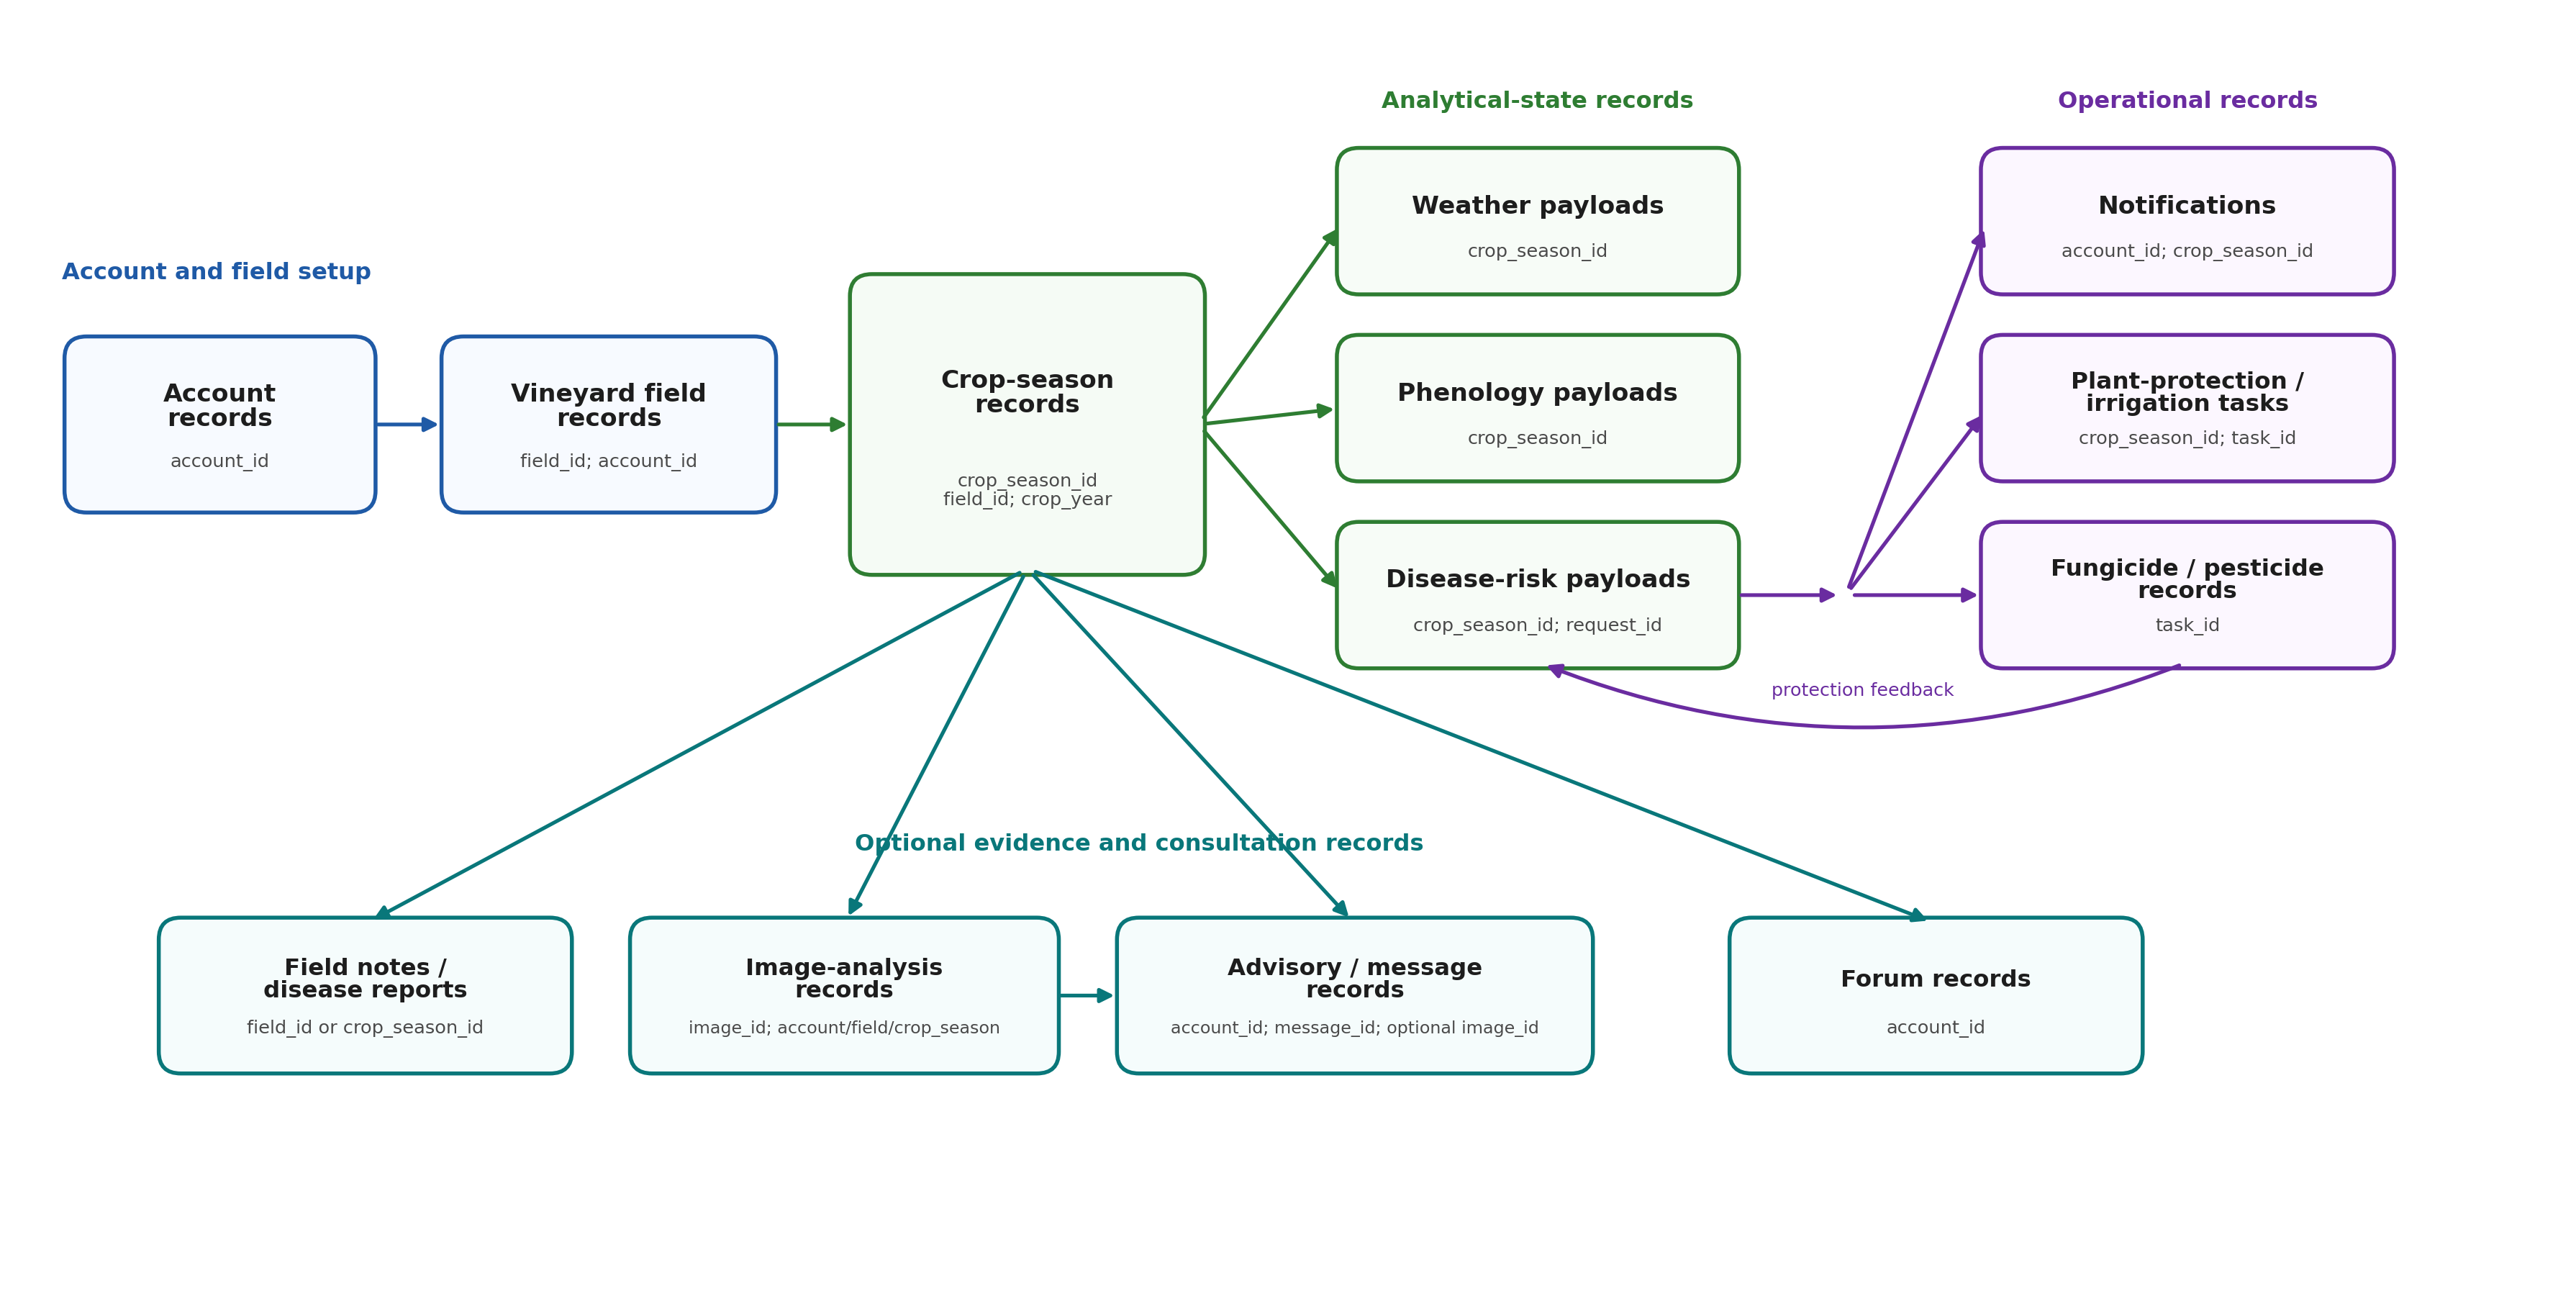
\includegraphics[width=\linewidth]{fig/grapemaster_backend_identifier_linkage.png}
\caption{Backend identifier relationships among GrapeMaster record classes. The crop record anchors the principal monitoring and management resources. Lines denote direct or contextual retrieval relationships according to the record type; they should not all be interpreted as direct foreign keys or causal provenance.}
\label{fig:supp_backend_operational_linkage}
\end{figure}

\begin{figure}[H]
\centering

\includegraphics[width=\linewidth]{fig/grapemaster_test_site_distribution_map.png}
\caption{Spatial context of mappable platform field records and independent experimental module-validation sites. Teal bubbles show mappable field records aggregated by region, with bubble size indicating the number of records per region. Red points indicate experimental sites used for module-level validation and are not part of the operational-record denominator.}
\label{fig:supp_platform_field_distribution}
\end{figure}

\section*{Supplementary tables}

\begingroup
\setlength{\tabcolsep}{3pt}
\renewcommand{\arraystretch}{1.12}
\begin{longtable}{@{}L{0.22\linewidth} L{0.37\linewidth} L{0.33\linewidth}@{}}
\caption{Input-output definitions and software roles of integrated analytical components.}\label{tab:supp_module_details}\\
\toprule
Service & Inputs and outputs & Invocation, workflow position, and evidence boundary \\
\midrule
\endfirsthead
\toprule
Service & Inputs and outputs & Invocation, workflow position, and evidence boundary \\
\midrule
\endhead
Weather service & Inputs include field coordinates and requested time windows. Outputs include historical and forecast weather plus derived spray-suitability variables. & The Django backend calls the Agromodel weather and geocoding service during initialization and scheduled refresh. Returned data are transformed and stored under crop-linked resources. \\
Phenology processing & Inputs include cultivar and crop metadata plus date-aligned daily temperature. Outputs include broad BBCH-related stage states and a daily stage sequence. & Runs as part of backend crop refresh and supplies both mobile display and host-state input for disease processing. The Guangxi result in the main paper supports the configured component. \\
Disease-risk service & Inputs include hourly weather, growth stage, cultivar susceptibility, target disease, and recent applied-fungicide history. Outputs include disease states, field risk, protection interpretation, recommendations, and treatment windows. & The stateless FastAPI service is called by Django; request and response are retained by the backend. The current source contains downy and powdery mildew paths. The FSIM-S result supports one platform-compatible Guangxi configuration but is not tied to every deployment record by an immutable version identifier. \\
Image-recognition service & Input is a user-selected symptom image. Output is hosted-service classification text and confidence information. & Called directly by the Flutter client as a post-symptomatic service. The service source and deployed checkpoint are outside the principal backend repository; seven-class performance is reported as supporting model evidence. \\
LLM-assisted advisory service & Inputs are user questions and diagnostic context available to the hosted advisory channel. Outputs are streamed management-oriented text terminated by an end marker. & Called over WebSocket by the Flutter client. The client contract is documented, but the hosted checkpoint, fine-tuning data, prompt, and version were not included in the available source. Advisory quality was not independently evaluated. \\
\bottomrule
\end{longtable}
\endgroup

\begingroup
\setlength{\tabcolsep}{3pt}
\renewcommand{\arraystretch}{1.12}
\begin{longtable}{@{}L{0.23\linewidth} L{0.36\linewidth} L{0.33\linewidth}@{}}
\caption{Database relationship rules supporting crop-season-centered traceability.}\label{tab:supp_database_relationship_rules}\\
\toprule
Relationship rule & Required linkage & Verification purpose \\
\midrule
\endfirsthead
\toprule
Relationship rule & Required linkage & Verification purpose \\
\midrule
\endhead
Account-to-field linkage & Retained account identifiers must link to at least one vineyard field record & Confirms that the account has an operational vineyard context rather than registration-only activity \\
Field-to-crop-season linkage & Each evaluated crop-season record must be linked to a field record through field or crop-season identifiers & Separates persistent field identity from season-specific analytical and management state \\
Crop-season-to-analytical-payload linkage & Weather, phenology, disease-risk, and model request-response payloads should share the crop-season identifier where applicable & Confirms that analytical inputs and outputs can be retrieved under the same seasonal anchor \\
Crop-season-to-event linkage & Notifications, warning events, and task records may be associated through retained user, field, or crop context & Supports contextual retrieval; a task does not store a dedicated source-notification foreign key, so event-to-task causality is not established \\
Task-to-product linkage & Fungicide or pesticide product records must link to plant-protection tasks through task identifiers & Confirms that completed operations can be converted into product-level treatment feedback \\
Crop-season-to-symptom/advisory record linkage & Image records, advisory records, field notes, and disease reports use the account, field, crop, image, or message identifiers available to each function & Supports functional association while acknowledging that advisory messages are primarily user- or message-keyed rather than uniformly crop-keyed \\
Explicit absence rule & If an expected optional record type is absent for a replay anchor, the absence is recorded rather than inferred as failure of unrelated workflow steps & Prevents overclaiming and separates missing symptom or advisory records from successful risk-task-feedback linkage \\
\bottomrule
\end{longtable}
\endgroup

\begingroup
\setlength{\tabcolsep}{3pt}
\renewcommand{\arraystretch}{1.12}
\begin{longtable}{@{}L{0.24\linewidth} L{0.36\linewidth} L{0.32\linewidth}@{}}
\caption{Rules used for the deployment-record demonstration and representative workflow reconstruction.}\label{tab:supp_verification_rules}\\
\toprule
Verification check & Operational criterion & Supported interpretation \\
\midrule
\endfirsthead
\toprule
Verification check & Operational criterion & Supported interpretation \\
\midrule
\endhead
Operational-account retention & An account is retained only when it has business records and field-crop-season linkage after deduplication and target-context screening & Defines the evaluated operational account set \\
Analytical payload completeness & A crop season is counted as analytically complete when weather, phenology, disease-risk, and request-response payloads are present under the shared seasonal context & Shows whether the analytical state can be reconstructed for that season \\
Disease-risk-to-operation context & Notification and task records are checked against retained user, field, or crop context & Shows whether event and operation objects coexist in the workflow context; it does not prove that one event caused one task \\
Treatment-feedback linkage & Fungicide or pesticide records are checked through task identifiers and task completion status & Shows whether field operations can be converted into feedback records \\
Symptom/advisory record-linkage availability & Image-analysis, advisory, disease-report, and note records are checked for available account, field, crop-season, image, or message links & Shows whether symptom-related records and advisory interactions are available for seasonal interpretation \\
Representative workflow & A selected crop anchor retrieves weather, phenology, disease-risk, notification, task, and fungicide records through shared crop or task keys & Illustrates the implemented risk-to-action-to-feedback objects and their available linkage strengths \\
Boundary reporting & Missing optional symptom or advisory records under the replay anchor are explicitly reported rather than omitted & Separates verified linkage from unsupported production-outcome claims \\
Excluded outcome claim & Operational-record linkage and replay checks are not treated as demonstrations of pesticide reduction, disease-control efficacy, economic benefit, or user adoption & Maintains the distinction between record-based workflow assessment and agronomic-impact evaluation \\
\bottomrule
\end{longtable}
\endgroup

\begingroup
\setlength{\tabcolsep}{3pt}
\renewcommand{\arraystretch}{1.12}
\begin{longtable}{@{}L{0.20\linewidth} L{0.29\linewidth} L{0.19\linewidth} L{0.22\linewidth}@{}}
\caption{Record-level reconstruction results for a representative GrapeMaster crop context.}\label{tab:supp_crop_season_replay_audit}\\
\toprule
Record group & Retained record set & Identifier or status & Result note \\
\midrule
\endfirsthead
\toprule
Record group & Retained record set & Identifier or status & Result note \\
\midrule
\endhead
Replay record set & Weather, phenology, disease-risk, notification, task, and fungicide records & One crop UUID & Representative workflow record set \\
State and risk records & Weather, phenology, and disease-risk payloads & Shared crop-season key & Shared seasonal record set \\
Operation records & Notifications and completed plant-protection tasks & Same crop context, without a direct source-notification task key & Contextual event and operation records \\
Treatment-feedback records & Fungicide-product records & Task identifiers & Product-task record set \\
Field-note branch & No field-note or incidence-note record & Explicit absence & No field/incidence note in this replay \\
\bottomrule
\end{longtable}
\endgroup

\begingroup
\setlength{\tabcolsep}{3pt}
\renewcommand{\arraystretch}{1.12}
\begin{longtable}{@{}L{0.20\linewidth} L{0.30\linewidth} L{0.42\linewidth}@{}}
\caption{Software stack and implementation components used in the GrapeMaster platform.}\label{tab:supp_software_stack}\\
\toprule
Layer & Component group & Main technologies or libraries \\
\midrule
\endfirsthead
\toprule
Layer & Component group & Main technologies or libraries \\
\midrule
\endhead
Mobile client & Application framework & Dart, Flutter \\
Mobile client & Android shell and build configuration & Kotlin, Gradle \\
Backend business service & Web framework and API layer & Python, Django 4.2, Django REST Framework \\
Backend business service & Authentication, scheduling, and asynchronous communication & SimpleJWT, Django APScheduler, Django Channels \\
Backend business service & Database access and persistence & PostgreSQL, \texttt{psycopg2}, normalized relational tables, JSON model payloads \\
Disease-model service & Service interface & FastAPI, Uvicorn, Pydantic, Starlette \\
Weather and time-series processing & Numerical and date-time processing & NumPy, Pandas, Python Dateutil, Pytz \\
Weather and geospatial processing & Field geometry, geocoding, and weather-service access & Shapely, Fiona, GeoPandas, Geopy, Requests, HTTPX, Agromodel weather/geocoding API, request caching, retry utilities \\
Phenology and risk analytics & Crop-stage and risk-state calculation & Python analytical workflows, date-aligned weather transformation, cultivar and crop-season metadata \\
Image processing and recognition & Image preprocessing and deep-learning inference & PyTorch, TorchVision, OpenCV, Pillow, Ultralytics-related components, EfficientViT-related modules, segmentation components \\
Advisory interface & Text advisory channel & Hosted WebSocket advisory service used by Flutter; concept follows the published CDIP-ChatGLM3 framework, while the deployed model artifact is externally maintained \\
\bottomrule
\end{longtable}
\endgroup

\begingroup
\setlength{\tabcolsep}{3pt}
\renewcommand{\arraystretch}{1.12}
\begin{longtable}{@{}L{0.23\linewidth} L{0.31\linewidth} L{0.38\linewidth}@{}}
\caption{Selected data-model attributes supporting the crop-season-centered workflow.}\label{tab:supp_data_model_attributes}\\
\toprule
Record group & Main attributes or stored content & Platform role \\
\midrule
\endfirsthead
\toprule
Record group & Main attributes or stored content & Platform role \\
\midrule
\endhead
Field record & User linkage, field name, area, GeoJSON boundary, centroid coordinates, administrative region, sharing state, deletion state, notice state, and generated field-boundary preview & Persistent spatial and ownership unit for vineyard management \\
Field geometry processing & Boundary parsing, boundary-image generation, area estimation, centroid calculation, and optional geocoding request & Converts user-defined field boundaries into location and display objects \\
Crop-season record & UUID, field linkage, grape cultivar, cultivation method, vine age, field coordinates, field size, cultivar metadata, and timestamps & Field-linked crop-management context for weather, phenology, risk, notifications, tasks, and products; explicit season year, start, end, and lifecycle state are not implemented \\
Master-data records & Grape variety, cultivar susceptibility, cultivation method, BBCH stage, disease type, fungicide, pesticide, and reminder rules & Controlled reference values for field, crop-season, task, risk, and advisory records \\
Model payload records & Weather, phenology, disease-risk, and request-response payloads stored with structured records & Preserves inputs and outputs for mobile display, recalculation, and audit \\
\bottomrule
\end{longtable}
\endgroup

\begingroup
\setlength{\tabcolsep}{3pt}
\renewcommand{\arraystretch}{1.12}
\begin{longtable}{@{}L{0.25\linewidth} L{0.43\linewidth} L{0.24\linewidth}@{}}
\caption{Operational-record screening rules used before summarizing deployed GrapeMaster records.}\label{tab:supp_screening_rules}\\
\toprule
Screening step & Rule & Rationale \\
\midrule
\endfirsthead
\toprule
Screening step & Rule & Rationale \\
\midrule
\endhead
User-record integration & User records were integrated using available user identifier, custom-user identifier, and phone-number fields. & Avoids duplicate counting of account-level records \\
Business-record filter & Accounts with no business records across field, crop-season, notification, task, fungicide or pesticide, advisory or message, forum, disease-report, and note tables were excluded. & Removes registration-only accounts from operational summaries \\
Field-crop-season linkage filter & Accounts without both field records and crop-season records were excluded. & Retains records that contain the principal setup objects used in the deployment demonstration \\
Target-context filter & A single account associated only with Linwei District was excluded. & Retains the intended vineyard deployment context for the descriptive record summary \\
Retained account set & Forty-seven accounts remained from 95 deduplicated accounts. & Defines the candidate account set used for operational-record coverage \\
\bottomrule
\end{longtable}
\endgroup

\begingroup
\setlength{\tabcolsep}{3pt}
\renewcommand{\arraystretch}{1.12}
\begin{longtable}{@{}L{0.22\linewidth} L{0.34\linewidth} L{0.34\linewidth}@{}}
\caption{Verified implementation evidence and remaining archival requirements.}\label{tab:supp_reproducibility_boundaries}\\
\toprule
Component & Verified in the documented source and records & Required for a submission-grade archive \\
\midrule
\endfirsthead
\toprule
Component & Verified in the documented source and records & Required for a submission-grade archive \\
\midrule
\endhead
Flutter client & Field, crop, weather, risk, task, product, image, report, and streamed advisory flows; fixed service endpoints and parsed response contracts & Versioned release, configurable endpoints, build instructions, sample configuration, and interface-contract tests \\
Django backend & REST resources, field/crop identifiers, scheduled weather refresh, weather/phenology/disease payload storage, notifications, tasks, product linkage, and treatment-history translation & Deployment configuration, database migration snapshot, environment template, scheduler deployment guidance, automated tests, and dependency lock \\
Disease service & FastAPI schema, stateless request execution, downy and powdery pathways, field-risk and recommendation outputs, and fungicide-history input & Immutable model configuration, tagged source release, regression fixtures, deployment-to-validation version mapping, and parameter provenance \\
Image service & Client HTTP request, result parsing, image-related application records, and supporting seven-class performance result & Hosted source, checkpoint, class mapping, preprocessing, endpoint schema, version identifier, and deployment instructions \\
LLM advisory & Client WebSocket request and streaming response behavior plus advisory/message records & Model checkpoint, fine-tuning or retrieval data description, prompt and system policy, endpoint schema, version identifier, safety evaluation, and deployment instructions \\
Operational records & Aggregated counts, crop-context linkage, task-to-product linkage, and one representative reconstruction & De-identification script, schema dictionary, reproducible extraction query, and archived derived demonstration dataset \\
\bottomrule
\end{longtable}
\endgroup
\end{document}
